% !TeX spellcheck = cs_CZ
{\tikzset{external/prefix={tikz/FYZI/}}
 \tikzset{external/figure name/.add={ch48_}{}}
%=========================== Kapitola: Rázy =======================================================
\chapter{Rázy}\label{fyz:IchapXLVIII}
\minitoc
  \section{Skládání dvou vln}\label{fyz:IchapXLVIIIsecI}
  \section{Záznějové tóny a modulace}\label{fyz:IchapXLVIIIsecII}
  \section{Postranní pásy}\label{fyz:IchapXLVIIIsecIII}
  \section{Lokalizované vlnové balíky}\label{fyz:IchapXLVIIIsecIV}
  \section{Amplitudy pravděpodobnosti pro částice}\label{fyz:IchapXLVIIIsecV}
  \section{Vlny v trojrozměrném prostoru}\label{fyz:IchapXLVIIIsecVI}
  \section{Normální kmity}\label{fyz:IchapXLVIIIsecVII}
  \section{Příklady a cvičení}\label{fyz:IchapXLVIIIsecVIII}

    \begin{figure}[ht!] %\ref{fyz_fig451}
      \centering
      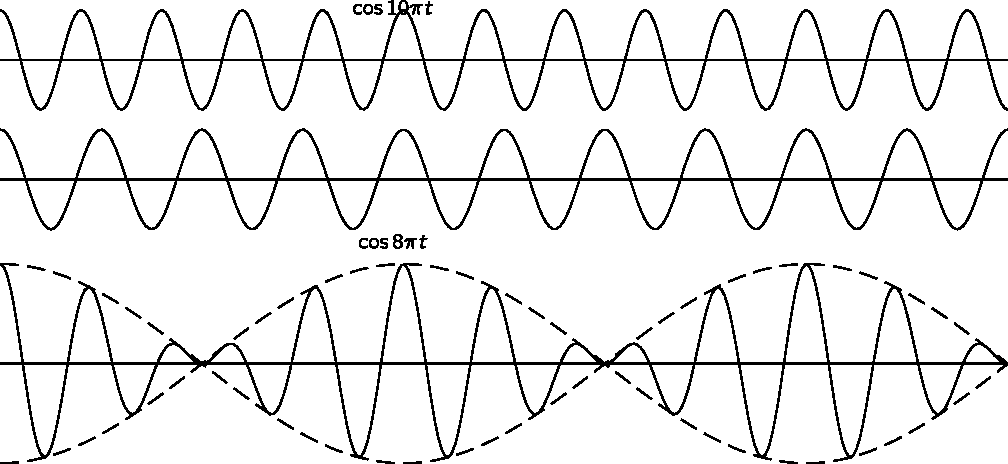
\includegraphics[width=0.7\linewidth]{fyz_fig451.pdf}
      \caption{ 
               (\cite[s.~707]{Feynman01})}
      \label{fyz_fig451}
    \end{figure}
    
    \begin{figure}[ht!] %\ref{fyz_fig452}
      \centering
      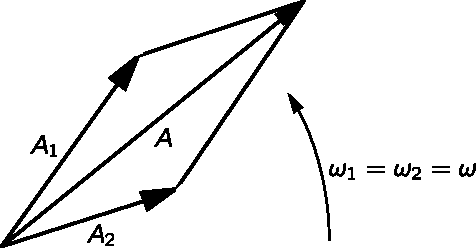
\includegraphics[width=0.7\linewidth]{fyz_fig452.pdf}
      \caption{ 
               (\cite[s.~707]{Feynman01})}
      \label{fyz_fig452}
    \end{figure}
    
    \begin{figure}[ht!] %\ref{fyz_fig453}
      \centering
      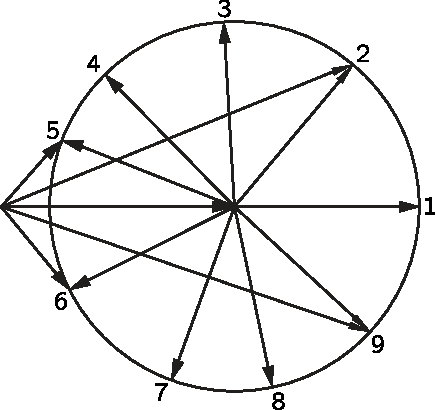
\includegraphics[width=0.7\linewidth]{fyz_fig453.pdf}
      \caption{ 
               (\cite[s.~707]{Feynman01})}
      \label{fyz_fig453}
    \end{figure}
    
    \begin{figure}[ht!] %\ref{fyz_fig454}
      \centering
      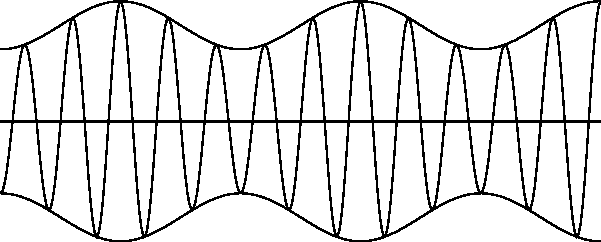
\includegraphics[width=0.7\linewidth]{fyz_fig454.pdf}
      \caption{ 
               (\cite[s.~707]{Feynman01})}
      \label{fyz_fig454}
    \end{figure}
    
    \begin{figure}[ht!] %\ref{fyz_fig455}
      \centering
      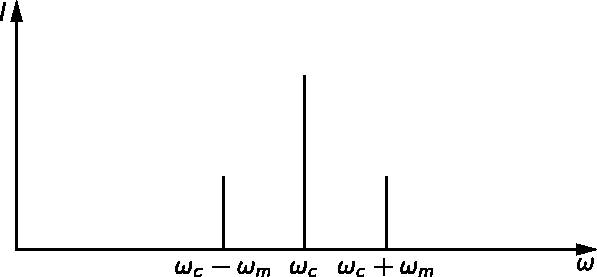
\includegraphics[width=0.7\linewidth]{fyz_fig455.pdf}
      \caption{ 
               (\cite[s.~707]{Feynman01})}
      \label{fyz_fig455}
    \end{figure}
    
    \begin{figure}[ht!] %\ref{fyz_fig456}
      \centering
      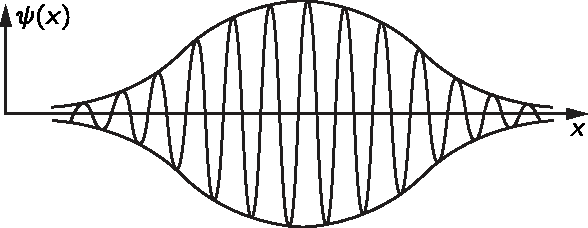
\includegraphics[width=0.7\linewidth]{fyz_fig456.pdf}
      \caption{ 
               (\cite[s.~707]{Feynman01})}
      \label{fyz_fig456}
    \end{figure}
    
} %tikzset
%---------------------------------------------------------------------------------------------------
\printbibliography[title={Seznam literatury}, heading=subbibliography]
\addcontentsline{toc}{section}{Seznam literatury}